 \documentclass[12pt]{article}
\usepackage{fullpage}
\usepackage{subfig}
\usepackage{blindtext}
\usepackage{graphicx}
\usepackage[font=small,labelfont=bf]{caption}
\usepackage{float}
\usepackage{textcomp}
\usepackage{hyperref}

\title{\textbf{\Huge Google Machine Learning Course}}
\date{\large July 2021}
\author{\Large Amaan Ahmad}
\begin{document}
\maketitle
\begin{abstract}
\begin{center}
	Machine Learning Crash Course with TensorFlow APIs Google's fast-paced, practical introduction to machine learning. Learn and apply fundamental machine learning concepts with the Crash Course, get real-world experience with the companion Kaggle competition, or visit Learn with Google AI to explore the full library of training resources.\\
	Course can be found \href{https://developers.google.com/machine-learning/crash-course}{here}
\end{center}

\end{abstract}
\newpage
\tableofcontents
\newpage
\section{Framing}
\subsection{Supervised Machine Learning}
The basic framework that will be explored is `Supervised Machine Learning'. Here, models are creates that combine inputs to produce useful predictions, even on previously unseen data.
\subsection{Labels}
A label is the target variable that is to be predicted — the y variable in simple \href{https://developers.google.com/machine-learning/glossary#linear_regression}{\textbf{linear regression}}. The label could be the future price of wheat, the kind of animal shown in a picture, the meaning of an audio clip, or just about anything.
\\ \newline In software such as a spam detector, the labels could include `spam' or `not spam'.
\subsection{Features}
Features are the way data is represented. A feature is an input variable — the x variable in simple \href{https://developers.google.com/machine-learning/glossary#linear_regression}{\textbf{linear regression}}. A simple machine learning project might use a single feature, while a more sophisticated machine learning project could use multiples of features, specified as: $x_1, x_2,...,x_n$
\\ \newline In a spam detector example, the features could include the following:
	\begin{itemize}
		\item email address
		\item words or phrases in the content of the email
		\item time of day that email was sent
	\end{itemize}
\subsection{Examples}
An `example' is a particular instance of data - such as one email. This could be either:
\begin{itemize}
	\item a \textbf{labelled example} - which has both feature information represented in the email and the label value of `spam' or `not spam'. These examples are used to \textbf{train} the model.
	\item an \textbf{unlabelled example} - which there is the feature information but no information on whether it is `spam' or `not spam'. These examples are used to \textbf{test} the model.
\end{itemize}
\subsection{Models}
A `model' defines the relationship between the features and the label and this is what is doing the predicting through a process of \textbf{learning} from data. \\\newline For example, with the spam detection model, the model may associate some features stronger with `spam' than others.
\\\newline There are two phases in a models life:
	\begin{itemize}
		\item \textbf{Training} - means creating or \textbf{learning} the model. In this phase, you show the model labelled examples to enable the model to gradually learn the relationships between features and label (x).
		\item \textbf{Inference} - means applying the trained model to unlabeled examples. Here, the trained model is used to make useful predictions (y).
	\end{itemize}
\subsection{Regression or Classification}
\begin{itemize}
	\item \textbf{Regression} models predicts continuous values (i.e. value of a house or probability).
	\item \textbf{Classification} models predict discrete values (i.e. if an email is `spam' or `not spam', or is an image a `dog', a `cat' or `horse').
\end{itemize}
\section{Descending into ML}
\subsection{Linear Regression}
For a linear relationship, we can model it using the equation for a line, which is:
\begin{center}
$y = mx + c$
\end{center}
However, in machine learning we use:
\begin{center}
$y' = w_1x_1 + b$
\end{center}
Where:
\begin{itemize}
	\item $y'$ is the predicted label - the output.
	\item $w_1$ is the weight of feature 1.
	\item $x_1$ is the feature.
	\item $b$ is the bias - also known as $w_0$.
\end{itemize}

This model only uses one feature however if we wanted to use multiple features, each feature would have a different weight and hence the formula would look like this:
\begin{center}
$y' = b + w_1x_1 + w_2x_2 + w_3x_3 + ... + w_nx_n$
\end{center}
\subsection{Training and Loss}
\href{https://developers.google.com/machine-learning/glossary#training}{\textbf{Training}} a model means determining good values for all the weights and the bias from labelled examples. In supervised learning, a machine learning algorithm determines a suitable model by examining many examples and attempting to find a model that minimizes loss - this process is called \textbf{Empirical Risk Minimization}.
\\ \href{https://developers.google.com/machine-learning/glossary#loss}{\textbf{Loss}} is the penalty of making a bad predictions. It is a number indicating how bad the model's prediction was on a single example. The goal of training a model is to find a set of weights and biases that have a \textit{low loss} on average with the aim of a perfect model having the loss of zero. Figure 1 demonstrates how a model attempted to find an appropriate model. Here the Arrowed lines represent the loss and the blue line represent the predictions.

\begin{figure}[h]
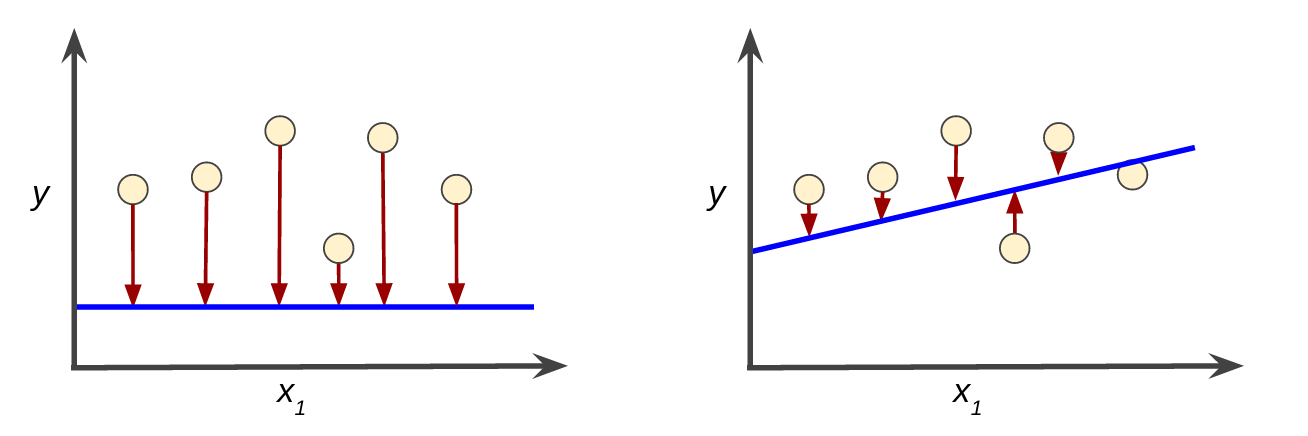
\includegraphics[scale = 0.3]{imgs/LossSideBySide}
\centering
\caption{Shows a high loss model (left) and a low loss model (right)}
\end{figure}
Mathematical functions — called \textbf{loss functions} — are used to aggregate the individual losses in a meaningful fashion.
\subsubsection{Squared Loss}
We use a loss function on linear regression called \textbf{Squared Loss}  (also known as \textbf{$L_2$ loss}). It is the square of the difference of the label and the prediction as shown by the equation:
\begin{center}
$(observation - prediction(x))^2$ or $(y - y')^2$
\end{center}

\subsubsection{Mean Square Error}
MSE is the average squared loss per example over the entire dataset. MSE is calculated but summing all the squared losses and then divide by the number of examples:

\begin{center}
\large $MSE = {{1}\over {N}} \sum_{(x,y)\in D} (y - prediction(x))^2$
\end{center}
Where:
\begin{itemize}
	\item $(x,y)$ is an example in which
	\begin{itemize}
	\item $x$ is the set of features that the model uses to make predictions.
	\item $y$ is the example's label.
	\end{itemize}
	\item $prediction(x)$ is a function of the weights and bias with the set of features $x$.
	\item $D$ is the data set which contain numerous labelled examples, which are $(x,y)$ pairs.
	\item $N$ is the number of examples in $D$.
\end{itemize}
Although MSE is commonly-used in machine learning, it is neither the only practical loss function nor the best loss function for all circumstances.

\section{Reducing Loss}
\subsection{Iterative Approach}
Similar to the \textit{Hot or Cold game} where we start with a guess then see what the loss is, then try another guess of model parameters, ($w_1$ and $b_1$), and see if you are closer to the smallest loss. Figure 2 shows use this process.
\begin{figure}[h]
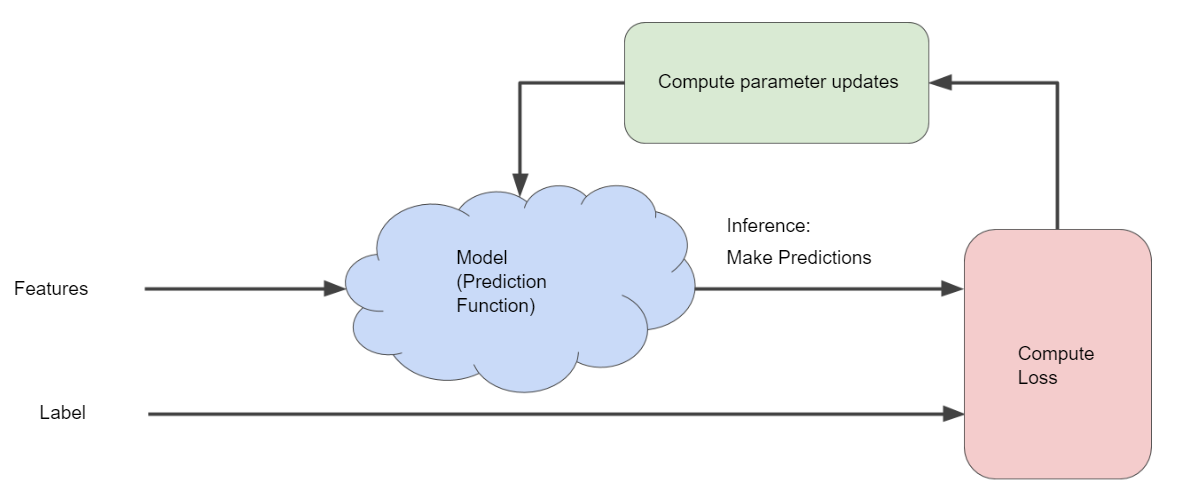
\includegraphics[scale = 0.5]{imgs/Iterative Approach.PNG}
\centering
\caption{Shows the trial and error approach which machine learning algorithms us to train the model}
\end{figure}
\\For example for a linear regression:
\begin{center}
$y' = w_1x_1 + b$
\end{center}

We choose random numbers for example;
$b = 0$ and $w_1 = 0$
The initial values we choose does not matter. We then get the predict value $y'$. Using this predicted value we use the loss function (finding the difference between y' and the correct label y corresponding to features x) to determine the loss. The program then iterates over to find the corresponding pair of values to find the lowest loss. Eventually, the loss stops changing (or at least changes extremely slowly) and this means the model \href{https://developers.google.com/machine-learning/glossary#convergence}{\textbf{converges}}. Iterative strategies are prevalent in machine learning, primarily because they scale so well to large data sets.
\subsection{Gradient Decent}
For linear regression problems, the resulting graph of loss vs $w_1$ will always be convex. which looks like this:

\begin{figure}[ht]
\centering
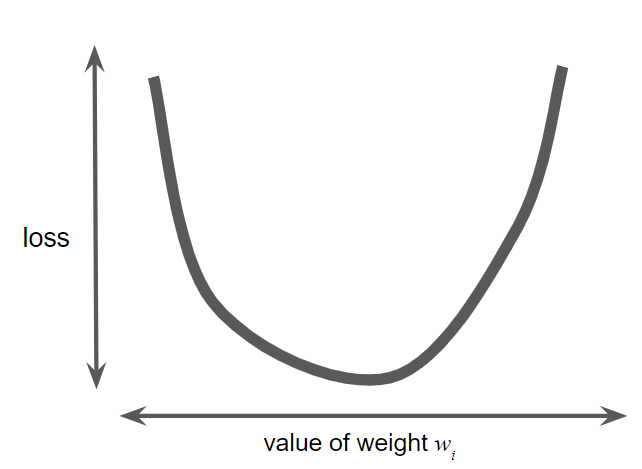
\includegraphics[scale = 0.7]{imgs/lossVSweight}
\caption{Shows the convex shaped graph}
\end{figure}

As shown in figure 3, we can see that the convex problem only has one minimum and this is where the loss function converges. To find the convergence point we use a mechanism called \href{https://developers.google.com/machine-learning/glossary#gradient_descent}{\textbf{gradient descent}}.
\\The algorithm picks a starting point (doesn't matter much so most algorithms set $w_1 = 0$), finds the gradient of the curve, then the algorithm takes a \href{https://developers.google.com/machine-learning/glossary#step}{\textbf{step}} in the direction of negative gradient to reduce loss. The gradient descent algorithm then calculates the gradient of the loss curve at the starting point. The gradient of the loss is equal to the derivative (slope) of the curve, and tells you which way is "warmer" or "colder." When there are multiple weights, the \textbf{gradient} is a vector of partial derivatives with respect to the weights. (Note: The gradient is a vector, so it has both direction and magnitude.) The gradient always points in the direction of steepest increase in the loss function. The gradient descent algorithm takes a step in the direction of the negative gradient in order to reduce loss as quickly as possible. To determine the next point along the loss function curve, the gradient descent algorithm adds some fraction (step) of the gradient's magnitude to the starting point. The value of this step is very important, as shown below in figure 4.

\begin{figure}[h]
\centering
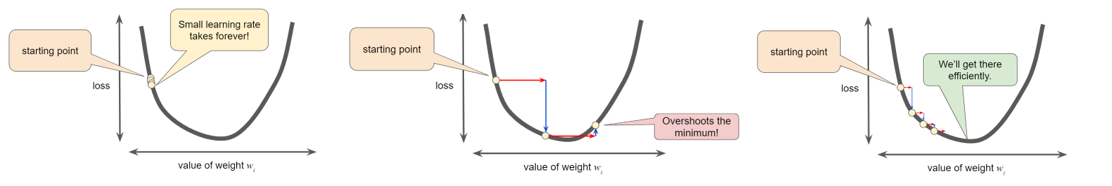
\includegraphics[scale = 0.85]{imgs/stepSize}
\caption{Left graph shows the small steps, Middle graph shows the effect of large steps and the Right graph shows the Goldilocks approach}
\centering
\end{figure}
When performing gradient descent, we generalize the above process to tune all the model parameters simultaneously. For example, to find the optimal values of both $w_1$ and the bias $b$, we calculate the gradients with respect to both $w_1$ and $b$. Next, we modify the values of $w_1$ and $b$ based on their respective gradients. Then we repeat these steps until we reach minimum loss. \\ 
The step size is also referred as the \textbf{learning rate}. Gradient descent algorithms multiply the gradient by this value to determine the next point. \textbf{Hyperparameters} are "knobs" that programmers tweak in machine learning algorithms to tune the learning rate.
As you can see from figure 4, if the learning rate is too small the learning would take too long. If the learning rate is to big, there is a possibility that you can overshoot the optimal point.
For every regression problem there is a Goldilocks learning rate which is related to how flat the loss funciton is. If the gradient of the loss function at the point is small then you can try a larger learning rate and vice-versa.

\subsection{Stochastic Gradient Descent - Reducing Loss}
In gradient descent, a \href{https://developers.google.com/machine-learning/glossary#batch}{\textbf{batch}} is the total number of examples you use to calculate the gradient in a single iteration. When working with large data sets, there are going to be huge numbers of features and as such even a single iteration can take a very long time to compute.
A large data set with randomly sampled examples probably contains redundant data. In fact, redundancy becomes more likely as the batch size grows.
\\\href{https://developers.google.com/machine-learning/glossary#SGD}{\textbf{Stochastic gradient descent (SGD)}} uses only a single example (a batch size of 1) per iteration. Given enough iterations, SGD works but is very noisy. The term "stochastic" indicates that the one example comprising each batch is chosen at random.
\\\href{https://developers.google.com/machine-learning/glossary#mini-batch}{\textbf{Mini-batch stochastic gradient descent (mini-batch SGD)}} is a compromise between full-batch iteration and SGD. A mini-batch is typically between 10 and 1,000 examples, chosen at random. Mini-batch SGD reduces the amount of noise in SGD but is still more efficient than full-batch.

\section{First Steps with TensorFlow}
\href{https://developers.google.com/machine-learning/glossary#TensorFlow}{\textbf{TensorFlow}} is an end-to-end open source platform for machine learning. TensorFlow is a rich system for managing all aspects of a machine learning system; however, this class focuses on using a particular TensorFlow API to develop and train machine learning models. See the \href{https://tensorflow.org/}{\underline{TensorFlow documentation}} for complete details on the broader TensorFlow system.

TensorFlow APIs are arranged hierarchically, with the high-level APIs built on the low-level APIs. Machine learning researchers use the low-level APIs to create and explore new machine learning algorithms. In this class, you will use a high-level API named tf.keras to define and train machine learning models and to make predictions. tf.keras is the TensorFlow variant of the open-source Keras API. Please note that use of tf.keras requires understanding of \href{https://numpy.org/}{\textbf{NumPy}} and \href{https://pandas.pydata.org/}{\textbf{pandas}}. For a brief recap view these \href{https://colab.research.google.com/github/google/eng-edu/blob/main/ml/cc/exercises/numpy_ultraquick_tutorial.ipynb?utm_source=mlcc&utm_campaign=colab-external&utm_medium=referral&utm_content=numpy_tf2-colab&hl=en}{\textbf{NumPy}} and \href{https://colab.research.google.com/github/google/eng-edu/blob/main/ml/cc/exercises/pandas_dataframe_ultraquick_tutorial.ipynb?utm_source=mlcc&utm_campaign=colab-external&utm_medium=referral&utm_content=pandas_tf2-colab&hl=en}{\textbf{pandas}} tutorials.
\\To see the code used in this section please refer to {\tt{code/FirstStepsWithTF}}.
\\The following figure shows the hierarchy of TensorFlow toolkits:

\begin{figure}[h]
	\centering
	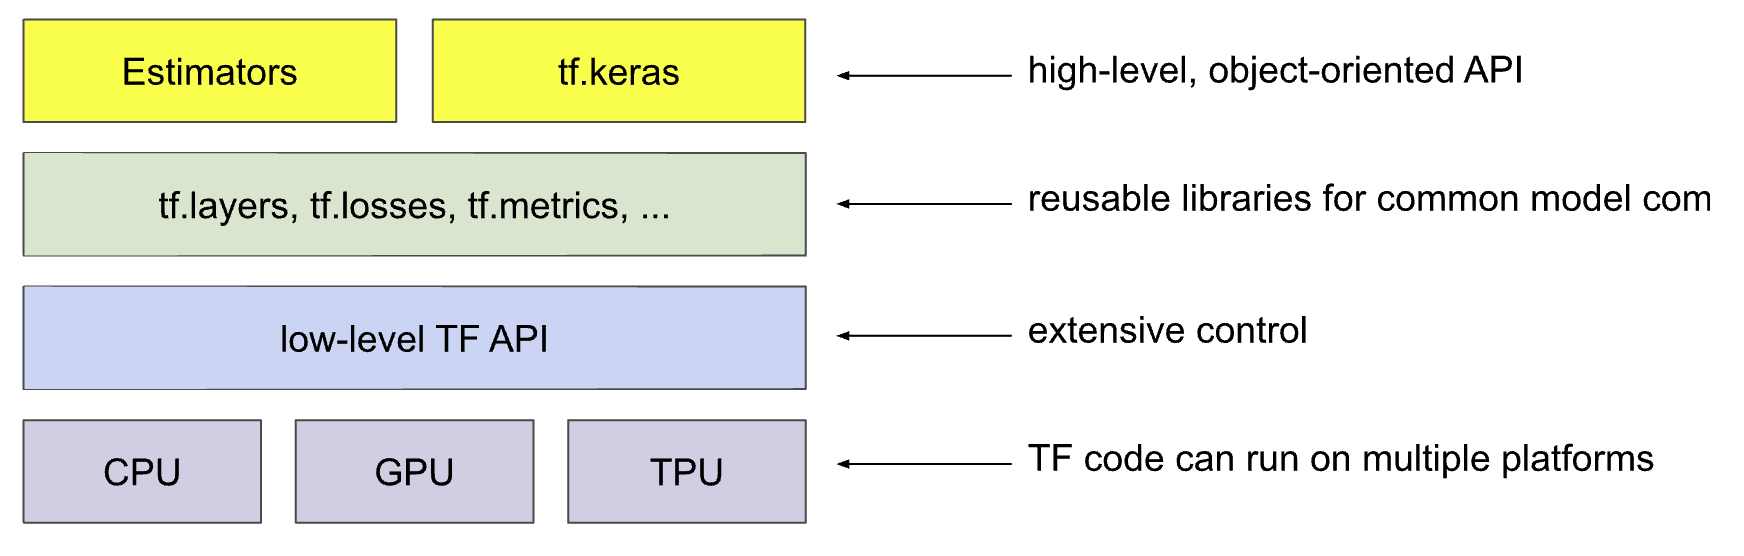
\includegraphics[scale = 0.55]{imgs/TFHierarchy.png}
	\caption{TensorFlow toolkit hierachy}
\end{figure}
\subsection{Summary of hyperparameter tuning}
Most machine learning problems require a lot of hyperparameter tuning. Unfortunately, we can't provide concrete tuning rules for every model. Lowering the learning rate can help one model converge efficiently but make another model converge much too slowly. You must experiment to find the best set of hyperparameters for your dataset. That said, here are a few rules of thumb:
\begin{itemize}
	\item Training loss should steadily decrease, steeply at first, and then more slowly until the slope of the curve reaches or approaches zero.
	\item If the training loss does not converge, train for more epochs.
	\item If the training loss decreases too slowly, increase the learning rate. Note that setting the learning rate too high may also prevent training loss from converging.
	\item If the training loss varies wildly (that is, the training loss jumps around), decrease the learning rate.
	\item Lowering the learning rate while increasing the number of epochs or the batch size is often a good combination.
	\item Setting the batch size to a very small batch number can also cause instability. First, try large batch size values. Then, decrease the batch size until you see degradation.
	\item For real-world datasets consisting of a very large number of examples, the entire dataset might not fit into memory. In such cases, you'll need to reduce the batch size to enable a batch to fit into memory.
\end{itemize}
Remember: the ideal combination of hyperparameters is data dependent, so you must always experiment and verify.

\subsection{Correlation Matrix}
A \textbf{correlation matrix} indicates how each attribute's raw values relate to the other attributes' raw values. Correlation values have the following meanings:
\begin{itemize}
	\item 1.0: perfect positive correlation; that is, when one attribute rises, the other attribute rises.
	\item -1.0: perfect negative correlation; that is, when one attribute rises, the other attribute falls.
	\item 0.0: no correlation; the two columns are not linearly related.
\end{itemize}
In general, the higher the absolute value of a correlation value, the greater its predictive power. 

\section{Generalisation}
The figure below shows the two graphs \href{https://developers.google.com/machine-learning/glossary#overfitting}{\textbf{overfit}} the traits of the data that the model was trained on. The model gets a low loss during training but does a poor job \href{https://developers.google.com/machine-learning/glossary#prediction}{\textbf{predicting}} new data as shown by the figure on the right.
\begin{figure}[h]%
    \centering
	\subfloat[A complex model for distinguishing sick from healthy trees.]{{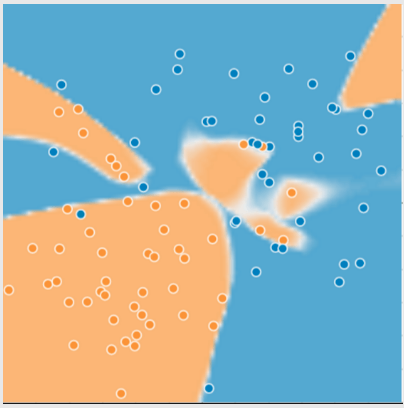
\includegraphics[width=7.5cm]{imgs/complexPredictionModel.png}}}%
    \qquad
    \subfloat[The model did a bad job predicting new data.]{{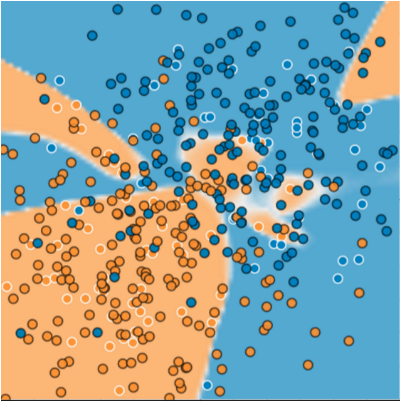
\includegraphics[width=7.5cm]{imgs/complexModelWithNewData.png}}}%
    \caption{}%
\end{figure}

Overfitting is caused by making a model more complex than necessary. The fundamental tension of machine learning is between fitting our data well, but also fitting the data as simply as possible.

\subsection{William of Ockham}
William of Ockham was a 14th century philosopher and loved simplicity. He believed that simpler formulae and theories are better than more complex ones. Thus in machine learning terms:
\begin{center}
	\textit{``The less complex an ML model, the more likely that a good empirical result is not just due to the peculiarities of the sample."}
\end{center}
In modern times, we've formalised Ockham's razor into the fields of \textbf{statistical learning theory} and \textbf{computational learning theory}. These fields have developed \textbf{generalisation bounds} - a statistical description of a model's ability to \href{https://developers.google.com/machine-learning/glossary#generalization}{\textbf{generalise}} to new data based on factors such as:
\begin{itemize}
	\item the complexity of the model
	\item the model's performance on training data
\end{itemize}
While the theoretical analysis provides formal guarantees under idealised assumptions, they can be difficult to apply in practice. Therefore, let's focus instead on empirical evaluation to judge a model's ability to generalise to new data.
A machine learning model aims to make good predictions on new, previously unseen data. But if you are building a model from your data set, how would you get the previously unseen data? Well, one way is to divide your data set into two subsets; 
\begin{itemize}
	\item \href{https://developers.google.com/machine-learning/glossary#training_set}{\textbf{training set}} - a subset to train a model
	\item \href{https://developers.google.com/machine-learning/glossary#test_set}{\textbf{test set}} - a subset to test the model
\end{itemize}
Good performance on the test set is a useful indicator of good performance on the new data in general, assuming that:
\begin{itemize}
	\item The test set is large enough.
	\item You don't cheat by using the same test set over and over.
\end{itemize}
\subsection{Machine Learning Fine Print}
There are three basic assumptions that aid generalisation:
\begin{itemize}
	\item Drawing examples \textbf{independantly and identically (i.i.d)} at random. This ensures the examples do not influence each other.
	\item The distribution is \href{https://developers.google.com/machine-learning/glossary#stationarity}{\textbf{stationary}} and so it doesn't change within the data.
	\item Drawing examples from partitions from the same distribution.
\end{itemize}

If the key assumptions of supervised ML are not met, then we lose important theoretical guarantees on our ability to predict on new data. However, in practise, we sometimes violate these assumptions.

\section{Training and Test Sets}
If you have a single data set, it is important to split the data into two subsets; the \href{https://developers.google.com/machine-learning/glossary#training_set}{\textbf{training set}} and the \href{https://developers.google.com/machine-learning/glossary#test_set}{\textbf{test set}}.
\\It is important that the test set is:
\begin{itemize}
	\item Large enough to get meaningful results
	\item Is representative of the data in the entire set.
\end{itemize}
\begin{figure}[h]
	\centering
	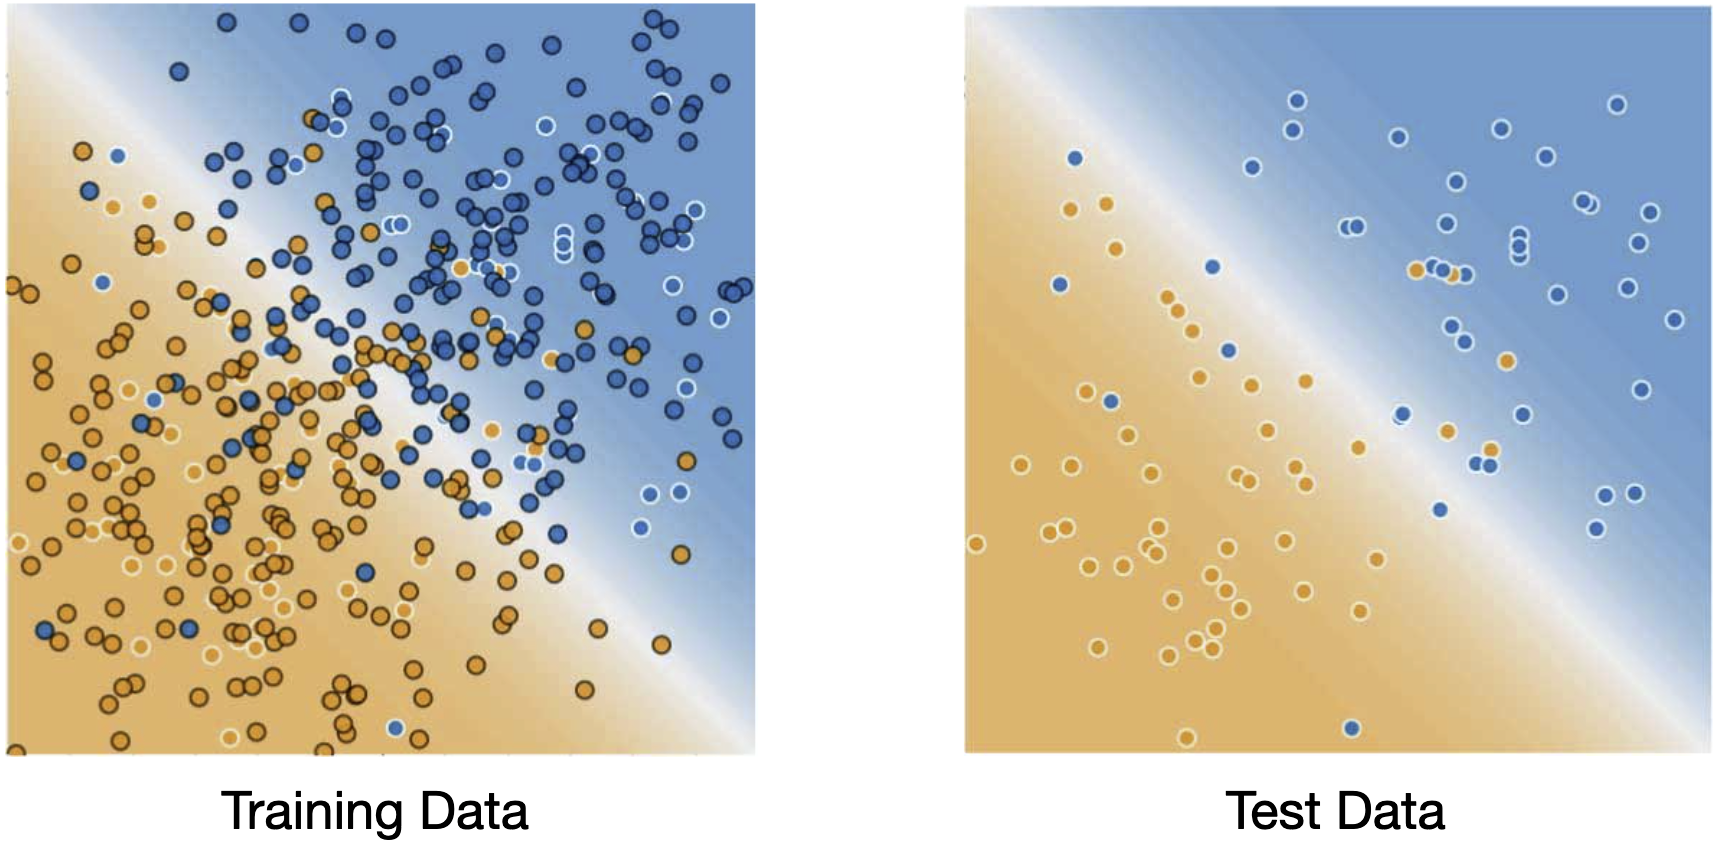
\includegraphics[scale = 0.5]{imgs/GoodTrainingAndTesting.png}
	\caption{Good example of a training and a testing set}
\end{figure}
Another important thing is that you must make sure that you never train the model using the test set as this gives you unrealistically strong opinions on how good your model is.
\section{Validation}
In the model mentioned previously, the dataset is split into 2 subsets as seen in \textbf{Figure \ref{fig: importance of validation sets}a}. However, this poseses a problem for us as the "Tweak Model", i.e. adjusting anything about the model (e.g. learning rate) to designing a new model, is evaluated against the test set and leads to easily overfitting. Due to this, we divide the set into 3 subsets as seen in 
\begin{figure}[h!]%
    \centering
	\subfloat[Workflow with two partitions of the dataset]{{\includegraphics[width=12cm]{imgs/PreValidation.png}}}%
    \qquad
    \subfloat[Workflow with three partitions of the dataset]{{\includegraphics[width=12cm]{imgs/PostValidation.png}}}%
    \caption{}%
	\label{fig: importance of validation sets}
\end{figure}
\textbf{Figure \ref{fig: importance of validation sets}b}. This has an improved workflow as it creates fewer exposures to the test set. As such we pick the model that does best on the new \href{https://developers.google.com/machine-learning/glossary#validation_set}{\textbf{validation set}} and double check the model against our test set.
This helps as the model is chosen based on the validation set and also that the model is double checked by the test set.

\section{Representaion}
\subsection{Feature Engineering}
The left side of \textbf{Figure \ref{fig: raw to feature}} demonstrates the raw data from the source and the right shows the \textbf{Feature Vector}, a set of float values.
\\\textbf{Feature Engineering} is the process in which raw data is transformed into a feature vector.
\begin{figure}[h]
	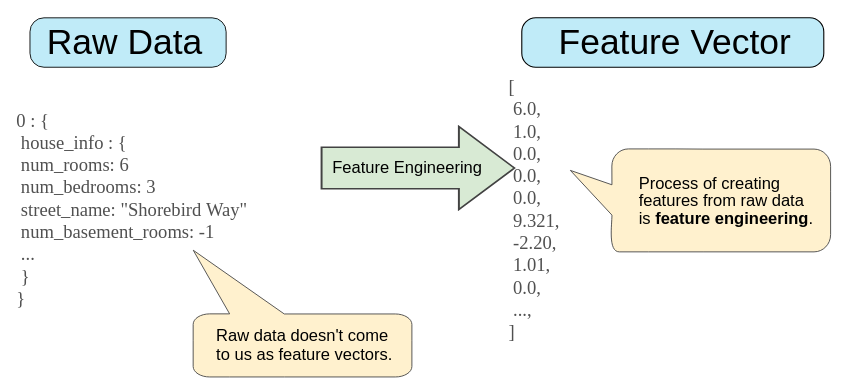
\includegraphics[scale = 0.5]{imgs/RawToFeature.png}
	\centering
	\caption{Feature Engineering example}
	\label{fig: raw to feature}
\end{figure}

\subsubsection{Mapping Numerical Values}
Mapping numerical values to floating-point is trivial as they can be multiplied by a numeric weight. The figure below gives an example.
\begin{figure}[h]
	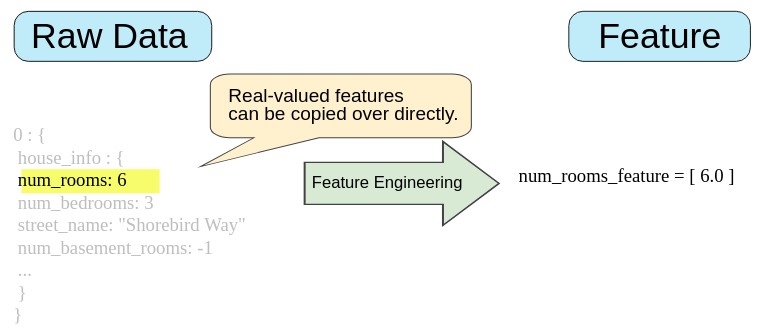
\includegraphics[scale = 0.5]{imgs/RawToIntFeature.png}
	\centering
	\caption{Mapping numerical values to floating point values}
\end{figure}

\subsubsection{Mapping Categorical Values} 
Mapping categorical is much less than mapping num'Makefile' has erical values. It is best described using an example:
\\
{\tt{\{'Charleston Road', 'North Shoreline Boulevard', 'Shorebird Way', 'Rengstorff Avenue'}\}}
\begin{figure}[h]
	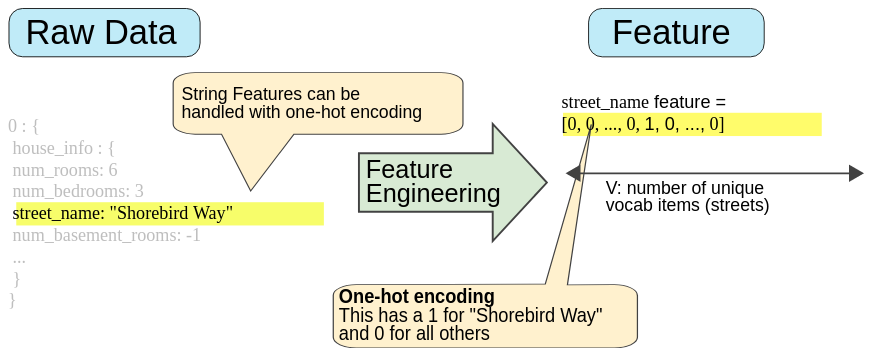
\includegraphics[scale = 0.5]{imgs/RawToStringFeature.png}
	\centering
	\caption{}
\end{figure}
\\We can accomplish this by defining a mapping from the feature values, which we'll refer to as the vocabulary of possible values, to integers. Since not every street in the world will appear in our dataset, we can group all other streets into a catch-all "other" category, known as an \textbf{OOV (out-of-vocabulary)} bucket.
\\Using this, we get:
\begin{itemize}
	\item Charleston Road = 0
	\item North Shoreline Boulevard = 1
	\item Shorebird Way = 2
	\item Rengstorff Avenue = 3
	\item Everything else (OOV) = 4
\end{itemize}
We then crete a binary vector for each categorical feature. So we set the corresponding vector elements to 1. And all other values to 0. However, multiple values could be set if necessary, this is called \textbf{multi-hot encoding}. If only a single value is set, it is called \textbf{one-hot encoding}. The figure above gives us an visual example.

\subsection{Ensuring a Good Representation of Features}
\subsubsection{Use Discrete Feature Values}
Having many discrete values would help the model see the feature in different situations, and thus would be able to determine when it is a good predictor.
For example, having {\tt{house\_type: victorian}} instead of {\tt{unique\_house\_id: 8SK982ZZ1242Z}}. Having the latter, would mean the model would not be able to learn anything from it as it would appear very rarly.
\subsubsection{Provide Obvious Meanings}
Each feature should give a clear meaning for example, having {\tt{house\_age\_years: 27}} instead of {\tt{house\_age: 851472000}}. This helps us find noisy data for example {\tt{user\_age\_years: 277}}, which is easier to spot that it this cannot be valid.
\subsubsection{Don't Mix Actual Data with "Magic Numbers"}
Floating point values should be in between 0 and 1, and if there is no value associated, e.g. if the user did not enter a value, then have a Boolean feature to specify if that feature is defines.
\subsubsection{Account for Potential Changes with the Meanings of Feature Values}
The meaning of the feature value should not change over time. For example, having {\tt{city\_lol: "london"}} instead of {\tt{inferred\_city\_cluster: "23"}}. As "london" is less likely to change in comparison to the meaning of "23".

\subsection{Cleaning Data}
\subsubsection{Scaling Feature Values}
Scaling means converting floating-point feature values from their natural range (for example, 100 to 900) into a standard range (for example, 0 to 1 or -1 to +1). In this way we avoid the model from inappropriately weighting features. 

\subsubsection{Handling Extreme Outliers}
For outliers, there are numberious ways to avoid this:

\begin{itemize}
	\item Logging the values - e.g. roomsPerPerson = log((totalRooms \/ population) + 1)
	\item Clipping, capping the values at a certain point - e.g. roomsPerPerson = min(totalRooms \/ population, 4)
\end{itemize}

\subsubsection{Binning}
Binning is grouping values together as shown below.
\begin{figure}[H]
	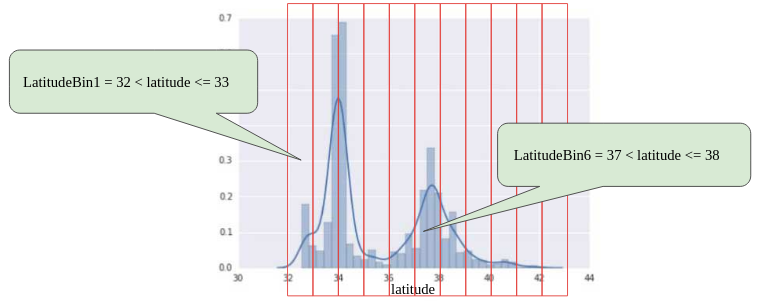
\includegraphics[scale = 0.5]{imgs/binning.png}
	\centering
	\caption{Binning Latitude}
\end{figure}
Instead of having one floating-point feature, we now have 11 distinct boolean features. Having 11 separate features is somewhat inelegant, so let's unite them into a single 11-element vector.

\subsubsection{Scrubbing}
Many examples in data sets are unreliable, and hence these values need to be removed from the set.
\begin{itemize}
	\item \textbf{Omitted Values} - If the user forgets to enter a value.
	\item \textbf{Duplicates}
	\item \textbf{Bad Labels} - Labelling errors.
	\item \textbf{Bad Feature Values} - Value errors e.g. adding an extra digit or a wrong one.
\end{itemize}
To find bad examples, a Histogram would be a good way to represent the data. Other statistics that would help find errors would be; Maximum, Minimum, Mean, Median and Standard Deviation.

\section{Feature Crosses}
If it is difficult to separate the categories in the model as shown in \textbf{Figure 11}, we create a feature cross. A \textbf{feature cross} is a synthetic feature that encodes nonlinearity in the feature space by multiplying two or more input features together. For example, if we had features $x_1$ and $x_2$, the feature cross, $x_3$, would be $x_3 = x_1 * x_2$.
\\This would mean the linear formula becomes: $y = b + w_1x_1 + w_2x_2 + w_3x_3$. Where the weights $w_1$, $w_2$ and $w_3$ are all learnt by the linear model.

\begin{figure}[H]
	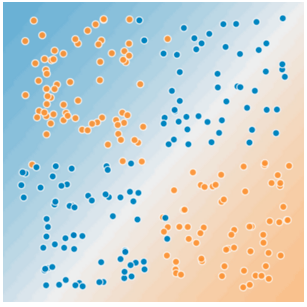
\includegraphics[scale = 0.5]{imgs/NonLinearModel.png}
	\centering
	\caption{Figure showing a non linear model }
\end{figure}

\section{Regularisation for Simplicity}
As you can see in \textbf{Figure 12} as you increase the iterations, the training loss decreases however the validation loss eventually begins to increase. This is because the model overfits to the given data. Up till now we have only been trying to decrease the training loss, now we will explore how we can avoid overfitting using a principle called regularisation.
\begin{figure}[H]
	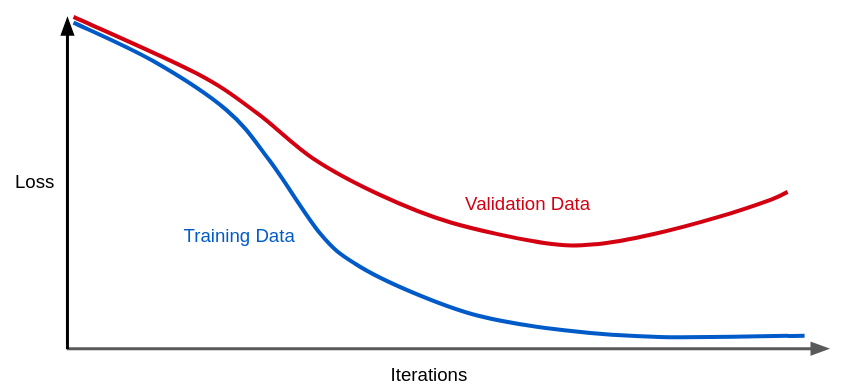
\includegraphics[scale = 0.5]{imgs/GeneralizationCurve.png}
	\centering
	\caption{Figure showing the generalization curve}
\end{figure}
We will now minimize the loss + complextity, this is called structural risk minimization:
\begin{center}
$minimize(Loss(Data|Model))$\\ \textrightarrow \\$minimize(Loss(Data|Model)) + complexity(Model)$
\end{center}
In this section, we will use the $L_2$ regularization, which quantifies the regularization term as the sum of squares of the feature wieghts.
\begin{center}
$L_2$ regularization term $= w^2_1 + w^2_2 + .. + w^2_n$
\end{center}
To further tune the impact of the regularization term. We multiply the $L_2$ value by a scalar, $\lambda$. Thus we now aim to: 
\begin{center}
$minimize(Loss(Data|Model)) + \lambda complexity(Model)$
\end{center}
In this way, the regularization ecourages weight values and the mean of the weights towards 0, with a Gaussian Distribution. Increasing the lambda value strengthens the regularization effect.
\begin{figure}[H]%
    \centering
	\subfloat[Histogram of weights with a high lamda value.]{{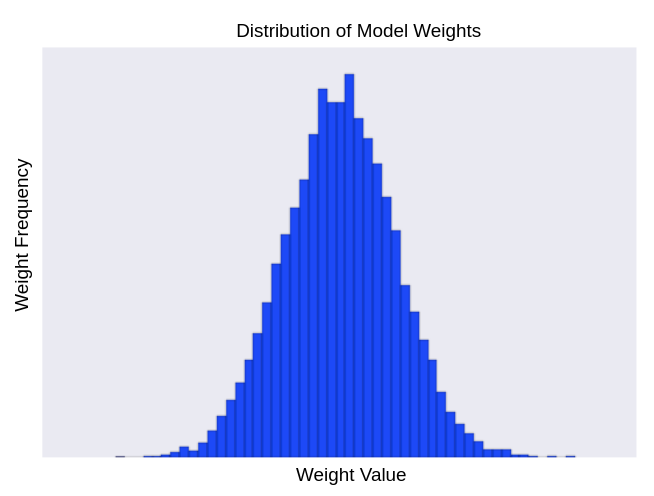
\includegraphics[width=7cm]{imgs/RegularizationNormDist.png}}}%
    \qquad
    \subfloat[Histogram of weights with a low lamda va'Makefile' has lue.]{{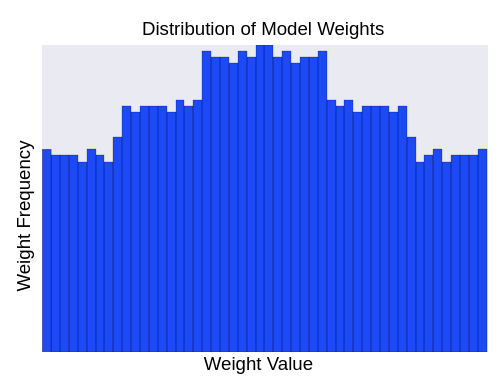
\includegraphics[width=7cm]{imgs/RegularizationBad.png}}}%
    \caption{Lowering the value of lambda tends to yield a flatter histogram}%
\end{figure}
If the lambda value is:
\begin{itemize}
\item too high, the model would be simple however there is a greater risk of underfitting the data. Hence the model would not be able to learn much from the training data.
\item too low, the model would be more complex however there is a greater risk of overfitting the data. This means it will learn too much about the particularities of the training data set.
\end{itemize}

\section{Logistic Regression}
There a two ways of calculating probability, "As is" and Converted to a binary category. The "As is" approach is self-explanatory. However, in classification cases we use a \textbf{sigmoid function}, which produces an output which always falls between 0 to 1. The sigmoid function is as follows:
\begin{center}
\begin{LARGE}
$y' = \frac{1}{1 + e^{-z}}$
\end{LARGE}
\end{center}
Where 
\begin{itemize}
\item $y'$ is the output of the logistic regression model for a particular example
\item $z = b + w_1x_1 + w_2x_2 + .. + w_Nx_N$
\end{itemize}
\subsection{Loss function for Logistic Regression}
The loss function for linear regression is squared loss. The loss function for logistic regression is Log Loss:
\begin{center}
\begin{LARGE}
$Log Loss = \sum_{(x, y) \in D}^{} -ylog(y') - (1 - y)log(1 - y')$
\end{LARGE}
\end{center}
Where 
\begin{itemize}
\item $(x,y) \in D$ is the dataset containing many labelled examples.
\item $y$ is the label in the label example. y is 0 or 1 as this is a logistic regression.
\item $y'$ is the predicted value, which is between 0 and 1.
\end{itemize}
\section{Classification}
\subsection{Thresholding}
Logistic regression returns a probability. We use the probability to predict how likely something is e.g. if an email was spam. We create a classification threshold to do the obvious, if its above a value then it is spam and if below it is not.
\subsection{True vs. False, Positve vs. Negative}
When predicting scenarios, there are four situations:
\begin{itemize}
\item True positive - when the model correctly predicts the positive class.
\item True negative - when the model correctly predicts the negative class.
\item False positive - when the model incorrectly predicts the positive class. 
\item False negative - when the model incorrectly predicts the negative class. 
\end{itemize}

\subsection{Accuracy, Precision and Recall}
\begin{center}
\begin{Large}
$Accuracy = \frac{Number\ of\ correct\ predictions}{Total\ number \ of\ predicitons}$
\linebreak\linebreak
$Precision = \frac{Number\ of\ True\ Positives}{Total\ number \ of\ Positive\ Predicitons}$
\linebreak\linebreak
$Recall = \frac{Number\ of\ True\ Positives}{Number \ of\ True \ Positives\ Predicitons\ and\ Number\ of\ False\ Negatives}$
\end{Large}
\end{center}

\subsection{ROC and AUC}
ROC curve (Receiver Operating Characteristic Curve) is a graph that shows the performance of a classifcation model, it has two parameters: True Positive Rate and False Positive Rate.
\begin{center}
\begin{Large}
$TPR = \frac{TP}{TP + FN}$
\linebreak\linebreak
$FPR = \frac{FP}{FP + TN}$
\end{Large}
\end{center}
The ROC pots TPR vs FPR at various classification decision thresholds.
\\ AUC is Area Under the ROC Curve. It provides a total performance measure over all classificatoin thresholds.
\begin{figure}[H]
	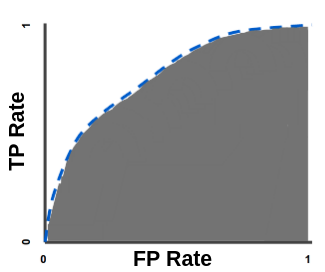
\includegraphics[scale = 0.5]{imgs/AUC.png}
	\centering
	\caption{Area Under the ROC Curve}
\end{figure}
AUC can be interpreted as the probability that the model ranks a random positive example more highly than a random negative example. Therefore, the closer the AUC to 1.0, the better as an AUC value of 1.0 means the predictions are 100\% correct.

\subsection{Prediction Bias}
Logistic regression predictions should be unbiased and this means:
\begin{center}
$average\ of\ predictions \approx average\ of\ observations$
\end{center}
The prediction bias is a the measure of how far apart the two are:
\begin{center}
$prediction\ bias\ =\ average\ of\ predictions - average\ of\ observations$
\end{center}

There are various causes of a prediction bias; Incomplete data set, Noisy data set, Buggy pipeline, Biased training sample or Over strong regularization. In order to correct the prediction bias by adding calibration layer. However, this could be problematic as you could be fixing symptoms rather than the cause or the system is brittle and you would need to constantly keep the model up-to-date.
\\
As the logistic regression model predicts a value between 0 and 1 however all labelled exapmles are either 0 or 1 therefore we can use "bucketing" to mitigate this issue. The are two ways to form buckets, linearly breaking up the target predictions or forming quantiles.\\ Consider the following calibration plot from a particular model. Each dot represents a bucket of 1,000 values. 
\begin{figure}[H]
	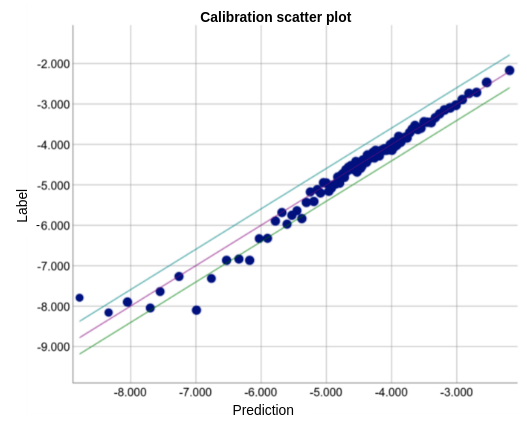
\includegraphics[scale = 0.3]{imgs/CalibrationScatter.png}
	\centering
	\caption{Area Under the ROC Curve}
\end{figure}

\section{Regularization: Sparsity}
Sparse vectors often contains many dimensions and creating a feature cross, creates even more dimensions. However, having numerous dimension features means when training the model, it becomes large and requires a lot of RAM.
\\In order to optimize the model we use regularization, however $L_2$ would not fix the issue as it does not force the weights to 0.0.
\\An apporoach we could take is $L_0$ regularization which is when chosen weights are reduced to 0 in order to be able to get the model to fit the data. However, this would turn our convex optimization problem into a non-convex optimization problem. 
\\An alternate is called $L_1$ regularization which means to make the noisy uninformative coefficients to 0 in order to create an approxi  mate to $L_0$  which saves a lot of RAM.

\section{Neural Networks}
A "non-linear" classification problem means that we can't accurately predict a label which has a model in the form of $b + w_1x_1 + w_2x_2$. For example:
\begin{figure}[H]
	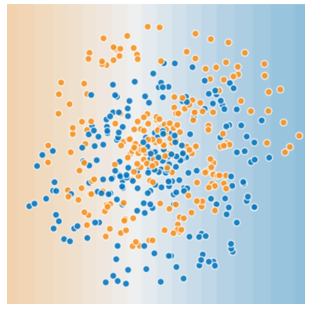
\includegraphics[scale = 0.5]{imgs/NonlinearComplex.png}
	\centering
	\caption{A Complex Nonlinear model}
\end{figure}
As you can see, we can't predict the model shown in \textbf{Figure 16} with a linear model. 
To begin understanding neural networks, let's visualize a linear model:
\begin{figure}[H]
	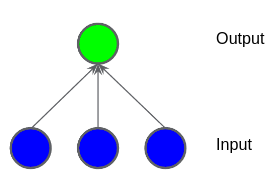
\includegraphics[scale = 0.5]{imgs/LinearGraph.png}
	\centering
	\caption{A Linear model as a graph}
\end{figure}
Each blue node represents an input feature and the green node which represents the weighted sum of the inputs.
\subsection{Hidden Layers}
We have now added a second layer to the model. The yellow nodes are the hidden layer which compute the weighted sum of the blue nodes and the green node computes the weighted sum of the yellow nodes. This model is still linear as it produces one output.
\begin{figure}[H]
	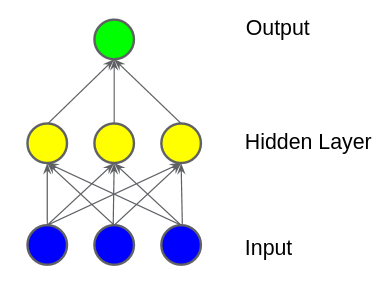
\includegraphics[scale = 0.5]{imgs/TwoLayerGraph.png}
	\centering
	\caption{Graph if a two-layer model}
\end{figure}
\subsection{Activation Functions}
To model a nonlinear problem, we can introduce nonlinearity. In the model below we see that Hidden Layer 1 is transformed by a nonlinear function before computing the weighted sum for the next layer. This nonlinear function is called the activation function.
\begin{figure}[H]
	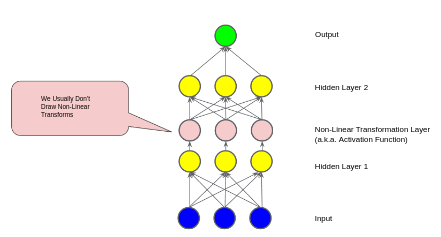
\includegraphics[scale = 0.5]{imgs/activationLayer.png}
	\centering
	\caption{Three-layer model with activation function}
\end{figure}
In this way we add more impact as stacking nonlinearities lets us model more complicated relationships.


\subsection{Common Activation Functions}

The sigmoid function converts the weighted sum to a value between 0 and 1.
\begin{center}
\begin{LARGE}
$F(x) = \frac{1}{1 + e^{-x}}$
\end{LARGE}
\end{center}
\vspace{1cm}
The \textbf{rectified linear unit} activation function (ReLU) works slightly better than the sigmoid "smooth" function.
\begin{center}
\begin{LARGE}
$F(x) = max(0,x)$
\end{LARGE}
\end{center}
However, any mathematical function can be an activation function.
\begin{center}
\begin{Large}
value of a node in the network $= \sigma(w \cdot x + b)$
\end{Large}
\end{center}
Where $\sigma$ represents our activation function e.g. sigmoid or ReLU.

\section{Best Practices when training neural networks}

\subsection{Failure Cases}

There are numerous ways backpropagation can go wrong.

\subsubsection{Vanishing Gradients}
Gradients for the layers closer to the input can be very small and when working with deep networks, the gradients could vanish towards 0.
\\The ReLU function can help mitigate this potential issue.
\subsubsection{Exploding Gradients}
If the weights are very large, the gradient of the lower layers involves products of many large terms. This overall means that the gradents become to large that they begin to converge.
\\We can use batch normalizations to prevent exploding gradients.
\subsubsection{Dead ReLU Units}
When the weighted sum for a ReLU falls below 0, the ReLU unit may get stuck. It then outputs 0 activation and thus the gradients become cut off. To avoid this we can lower the learning rate.
\subsection{Dropout Regularization}
Another type of regularization is Dropout regularization. It works by randomly dropping unit activations in a network for a single gradient step. The more you drop, the stronger the regularization. 0.0 = No dropout regularization and 1.0 = Drop out everything which means model learns nothing.



















\end{document}